\documentclass{article}

\usepackage{a4wide}
\usepackage[utf8]{inputenc}
\usepackage[T1]{fontenc}
\usepackage[french]{babel}
\usepackage[babel=true]{csquotes} % guillemets français
\usepackage{graphicx}
\graphicspath{{Images/}}
\usepackage{color}
\usepackage{hyperref}
\hypersetup{colorlinks,linkcolor=,urlcolor=blue}

\usepackage{amsmath}
\usepackage{amssymb}
\usepackage{natbib}


\title{Rapport de projet : File d'entiers en Java et en Python}
\author{\'Nativel Emmanuel, L3 informatique}
\date{\today}

\begin{document}

\maketitle % pour écrire le titre


%% Le résumé:
\begin{abstract}
  Construction d'un programme qui crée une file d’entiers de capacité maximale 20 ainsi qu’un thread producteur et plusieurs threads consommateurs se partageant cette file. Ces threads répètent indéfiniment les actions suivantes.
  — [Producteur] Ajout d’un entier choisi aléatoirement entre 1 et 100 puis repos. Si la file est pleine, ce thread est mis en attente jusqu’à ce qu’une place soit disponible.
  — [Consommateurs] Retrait d’un entier, affichage de cet entier puis repos. Si la file est vide, le thread est mis en attente jusqu’à ce qu’un entier soit disponible.
\end{abstract}

\section{Introduction}
\label{section:introduction}

Ce rapport est un descriptif d'une application créée dans le cadre de l'UE programmation concurrente. Elle a pour but de modéliser une file dans laquelle des entiers seront ajoutés et retirés indéfiniement. Pour que toutes ces actions se fassent "en même temps", nous allons utiliser plusieurs threads. Les languages utilisés sont Java et Python. Enfin, concernant l'interface graphique, nous allons utiliser la bibliothèque Swing\cite{swingDoc} en java et TKinter\cite{tkinterDoc} en python.

\section{Architecture générale de l'application}
\label{section:architecture}

L'application est composée de 4 classes :
\begin{itemize}
\item Thread \textbf{Consommateur} : Retire un entier dans la liste puis se met en repos. Si la file est vide, le thread est mis en attente jusqu’à ce qu’un entier soit disponible.
\item Thread \textbf{Producteur} : Ajout d’un entier choisi aléatoirement entre 1 et 100 puis se met en repos. Si la file
est pleine, ce thread est mis en attente jusqu’à ce qu’une place soit disponible.
\item La classe \textbf{Queue} : Modélise la file d'entiers. Cette classe contient les fonctions synchronisées qui agissent sur la file.
\item La classe \textbf{Fenêtre} : Contient l'interface graphique de l'application.
\end{itemize}

\cleardoublepage

\section{Captures d'écran}
\label{section:capture}

Interface graphique en Java :
\begin{center}
  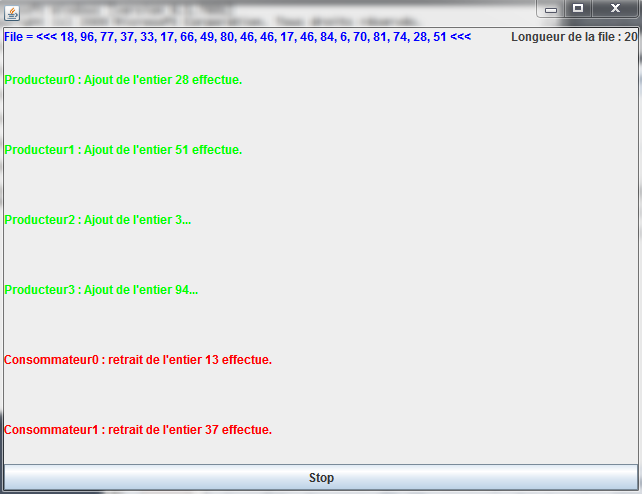
\includegraphics[scale=0.8]{java.PNG}
\end{center}

\cleardoublepage
Interface graphique en Python\cite{tkinterOpenClassroom} :
\begin{center}
  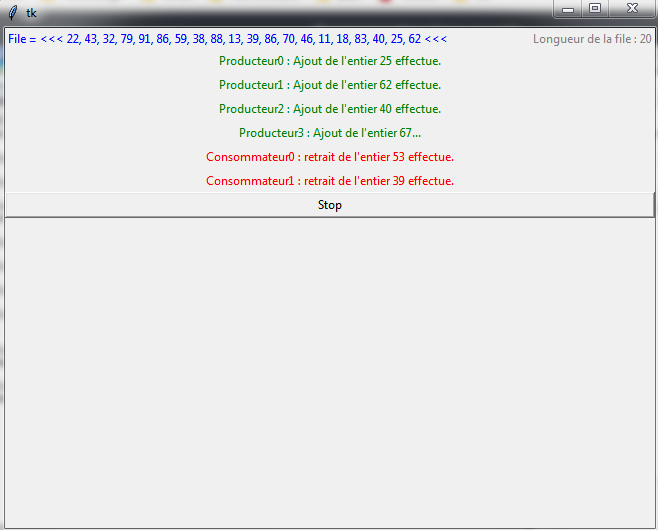
\includegraphics[scale=0.8]{python.PNG}
\end{center}

\section{Description de l'application}
\label{section:fonctionnement}
    \textit{Les explications qui suivent se basent sur la version java du programme. En ce qui concerne la version python, le fonctionnement est similaire, à l'exception de quelques points, comme l'interruption des threads et les évènements liés à l'interface graphique.}

\subsection{Fonctionnement de l'application}

Lorsque le bouton start est enclenché, la fonction create\_process() est appelée dans un premier temps. Elle se charge de créer le nombre d'objets producteurs et consommateurs demandés et les stocke dans des tableaux.
Dans un second temps, la fonction start\_process() parcourt les tableaux et lance la méthode start() des différents threads.
Enfin, le texte du bouton start est modifié et devient "stop".

Au départ, la file est vide. Les Threads producteurs et consommateurs commencent leurs actions et la liste se remplit, ou pas, petit à petit jusqu'à atteindre sa taille maximale.

Lorsque le bouton stop est enclenché, la fonction stop\_process() est lancée et parcourt à son tour les tableaux de threads et lance leur méthode interrupt().
Suite à cela, le bouton est désactivé. Il n'est donc plus possible de relancer le programme.

\cleardoublepage

\subsection{Description de quelques fonctions}
    \textbf{La fonction createString() : }
        \begin{verbatim}
              public synchronized String createString(){
                String s = "<<< ";
                for(int i=0; i<this.valeurs.size(); i++){
                  s+=String.valueOf(this.valeurs.get(i));
                  if(i!=this.valeurs.size()-1) s+=", ";
                }
                s+=" <<<";
                this.l_taille.setText("Longueur de la file : "+this.valeurs.size());
                return s;
              }
        \end{verbatim}

        Cette fonction a pour but de créer la chaîne de caractères correspondante à la file d'entiers et à l'affichage du nombre d'entiers contenus dans la file. La chaîne de caractères est construite petit à petit en parcourant le tableau qui stocke les entiers de la file. Cette méthode est synchronisée afin que les valeurs à afficher restent fixes pendant que l'affichage est en cours.
        \bigskip

    \textbf{La fonction majLabel() : }
        \begin{verbatim}
              private void majLabel(){
                this.l_liste.setText("File = "+this.createString());
                this.l_liste.repaint();
                this.l_taille.repaint();
              }
        \end{verbatim}

        La fonction majlabel() regroupe les actions à faire afin d'actualiser l'affichage de la file d'entiers. Premièrement, elle met à jour le texte du label. La fonction createString() va recréer la chaîne de caractères de la file avec les bons entiers.
        Puis, les labels l\_liste, qui contient la file d'entier, et l\_taille, qui contient une chaîne de caractères affichant la taille de la liste, sont actualisés grâce à l'appel de la méthode repaint().
        \bigskip

    \textbf{Détection des cliques sur le bouton : }
        \begin{verbatim}
            public void actionPerformed(ActionEvent e){ //Ce qui se passe quand on appuie sur le boutton
                Object source = e.getSource(); //Contient l'indentité de l'objet qui a enclenché l'évènement
                if(source instanceof JButton){
                  JButton bt_source = (JButton) source;
                  String titre = bt_source.getText();

                  switch(titre){
                    case "Start" : //actions lors de l'appuie sur le bouton start
                      create_process();
                      start_process();
                      bt_source.setText("Stop");
                      break;
                    case "Stop" : //actions lors de l'appuie sur le bouton stop
                      stop_process();
                      bt_source.setText("Start");
                      bt_source.setEnabled(false);
                      break;
                  }}}
        \end{verbatim}

        La distinction entre le bouton start et stop se fait grâce au texte du bouton, récupéré grâce à la méthode getText().
        \bigskip

    \textbf{La fonction enfiler() : }
        \begin{verbatim}
            public synchronized void enfiler(int n) throws InterruptedException{
                while(this.valeurs.size() == this.capacite) wait();
                this.valeurs.add(n);
                this.majLabel();
                notifyAll();
              }
        \end{verbatim}

        Cette fonction est mise en attente lorsque la file est pleine. Dans le cas contraire, elle ajoute à la file un entier aléatoire entre 1 et 100, puis met à jour l'affichage de la file par l'appel de la fonction majLabel() et termine par la fonction notifyAll() qui signale aux autres fonctions synchronisées qu'elle a terminé son exécution.
        \bigskip

    \textbf{La fonction defiler() : }
        \begin{verbatim}
            public synchronized int defiler() throws  InterruptedException {
                while(this.valeurs.size() == 0) wait();
                    int n = this.valeurs.removeFirst();
                    this.majLabel();
                    notifyAll();
                    return n;
            }
        \end{verbatim}

        Cette fonction est mise en attente lorsque la file est vide. Son fonctionnement est similaire à la fonction enfiler(), sauf qu'à la place d'ajouter un entier dans la file, elle retire le premier entier de la file.
        \bigskip

\cleardoublepage

\subsection{Organisation des interfaces graphiques}
Python :
\begin{center}
  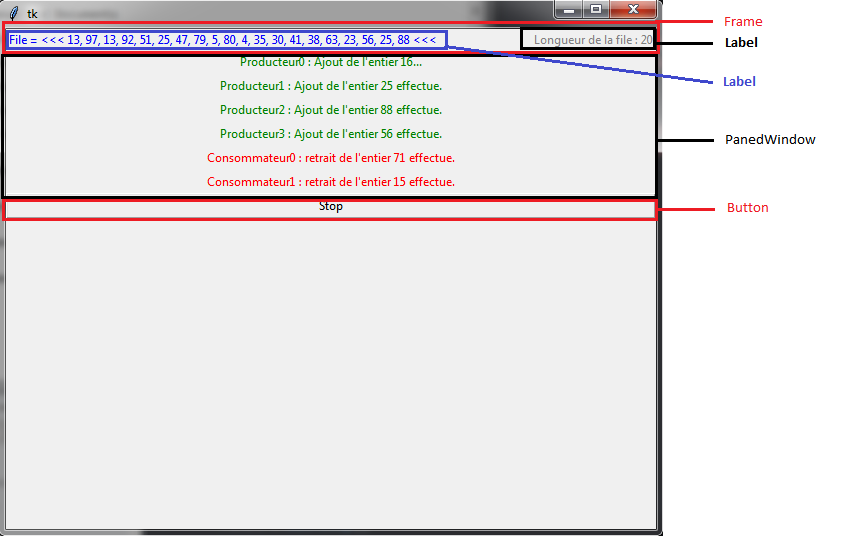
\includegraphics[scale=0.8]{zonesPython.PNG}
\end{center}

\cleardoublepage

Java :
\begin{center}
  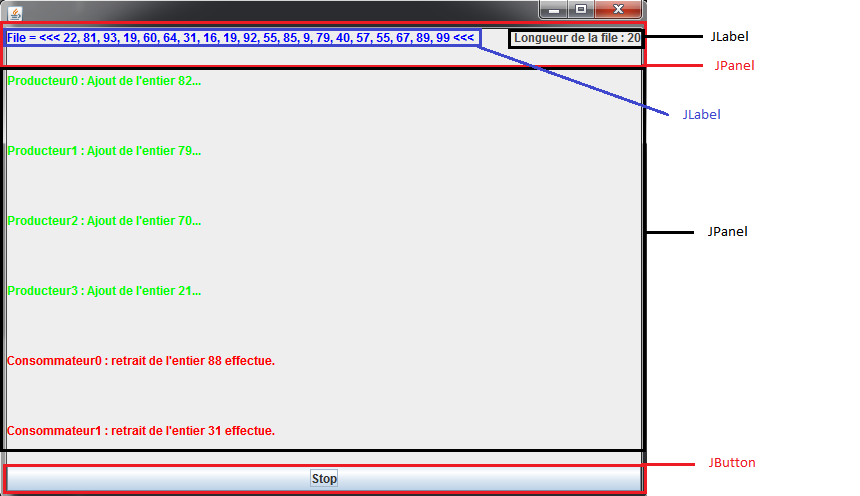
\includegraphics[scale=0.8]{zonesJava.PNG}
\end{center}

\section{Difficultés rencontrées}
\label{section:difficultées}
Les principales difficultés que j'ai rencontrées dans cet exercice étaient au niveau de l'interface graphique.
Premièrement, dans sa conception, le plus compliqué était de faire le lien entre les différentes classes et la classe dédiée à l'interface graphique. Par exemple, comment transmettre une information à afficher, dans quelle classe placer la fonction, ect...
Enfin, j'ai passé une grande partie de mon temps de travail dans les tutoriels et les documentations de Tkinter et de java Swing, notamment pour placer les objets dans la fenêtre.


\section{Conclusion}
\label{section:conclusion}
Pour conclure, le mécanisme de synchronisation des threads fonctionne, et l'affichage des états des threads également. Cependant, il aurait été intéressant d'ajouter un bouton pour mettre en pause l'exécution des threads, et de reprendre là où ils s'étaient arrêtés. Cela aurait pu se faire par l'intermédiaire d'une variable booléenne qui aurait été testée dans la boucle while des méthodes run() par exemple. Des améliorations graphiques sont évidemment envisageables.

\bibliographystyle{plain}
\bibliography{ma_biblio}

\end{document}
